\subsection{Section Objective}
The problem statement is the most important part of your paper and should be written first. First, allude to a diagram that shows the information flow with mathematical notation for your problem, such as Figure 2.
Then, systematically introduce key notation that helps you build up to a \textbf{formal mathematical optimization problem} with a cost function and constraints (in most problems our lab will focus on).

For a control or networking problem, describe the information flow. 
Namely, the sensory input, each computation function, and each function's input and output and task. Be formal, but provide a one sentence example for each.

\begin{enumerate}
    \item The sensory input.  Give the variable, an example,  and (during the first introduction) describe its dimension. ``\SC{The robot measures an n-dimensional sensory input $s_t \in \reals^n$, such as an image or LIDAR point cloud, at discrete time $t$.}''
    \item The controller's state space.
    \item The action space.
    \item The dynamics.
    \item The cost function.
\end{enumerate}

\subsubsection{Formal Problem Statement}
This should be in a formal problem statement block, such as in \cite{cheng2021data,nakanoya2021task}.
The statement should describe the inputs (``givens''), the optimization objective, and constraints. For the inputs and constraints, you likely will reference equations defined earlier. 

\subsubsection{Significance of the Problem}
Describe in one short paragraph why the problem is novel compared to state-of-the-art, how it broadly applies to many engineering settings, and what technical parts make it challenging to solve.

\begin{figure}
\centering
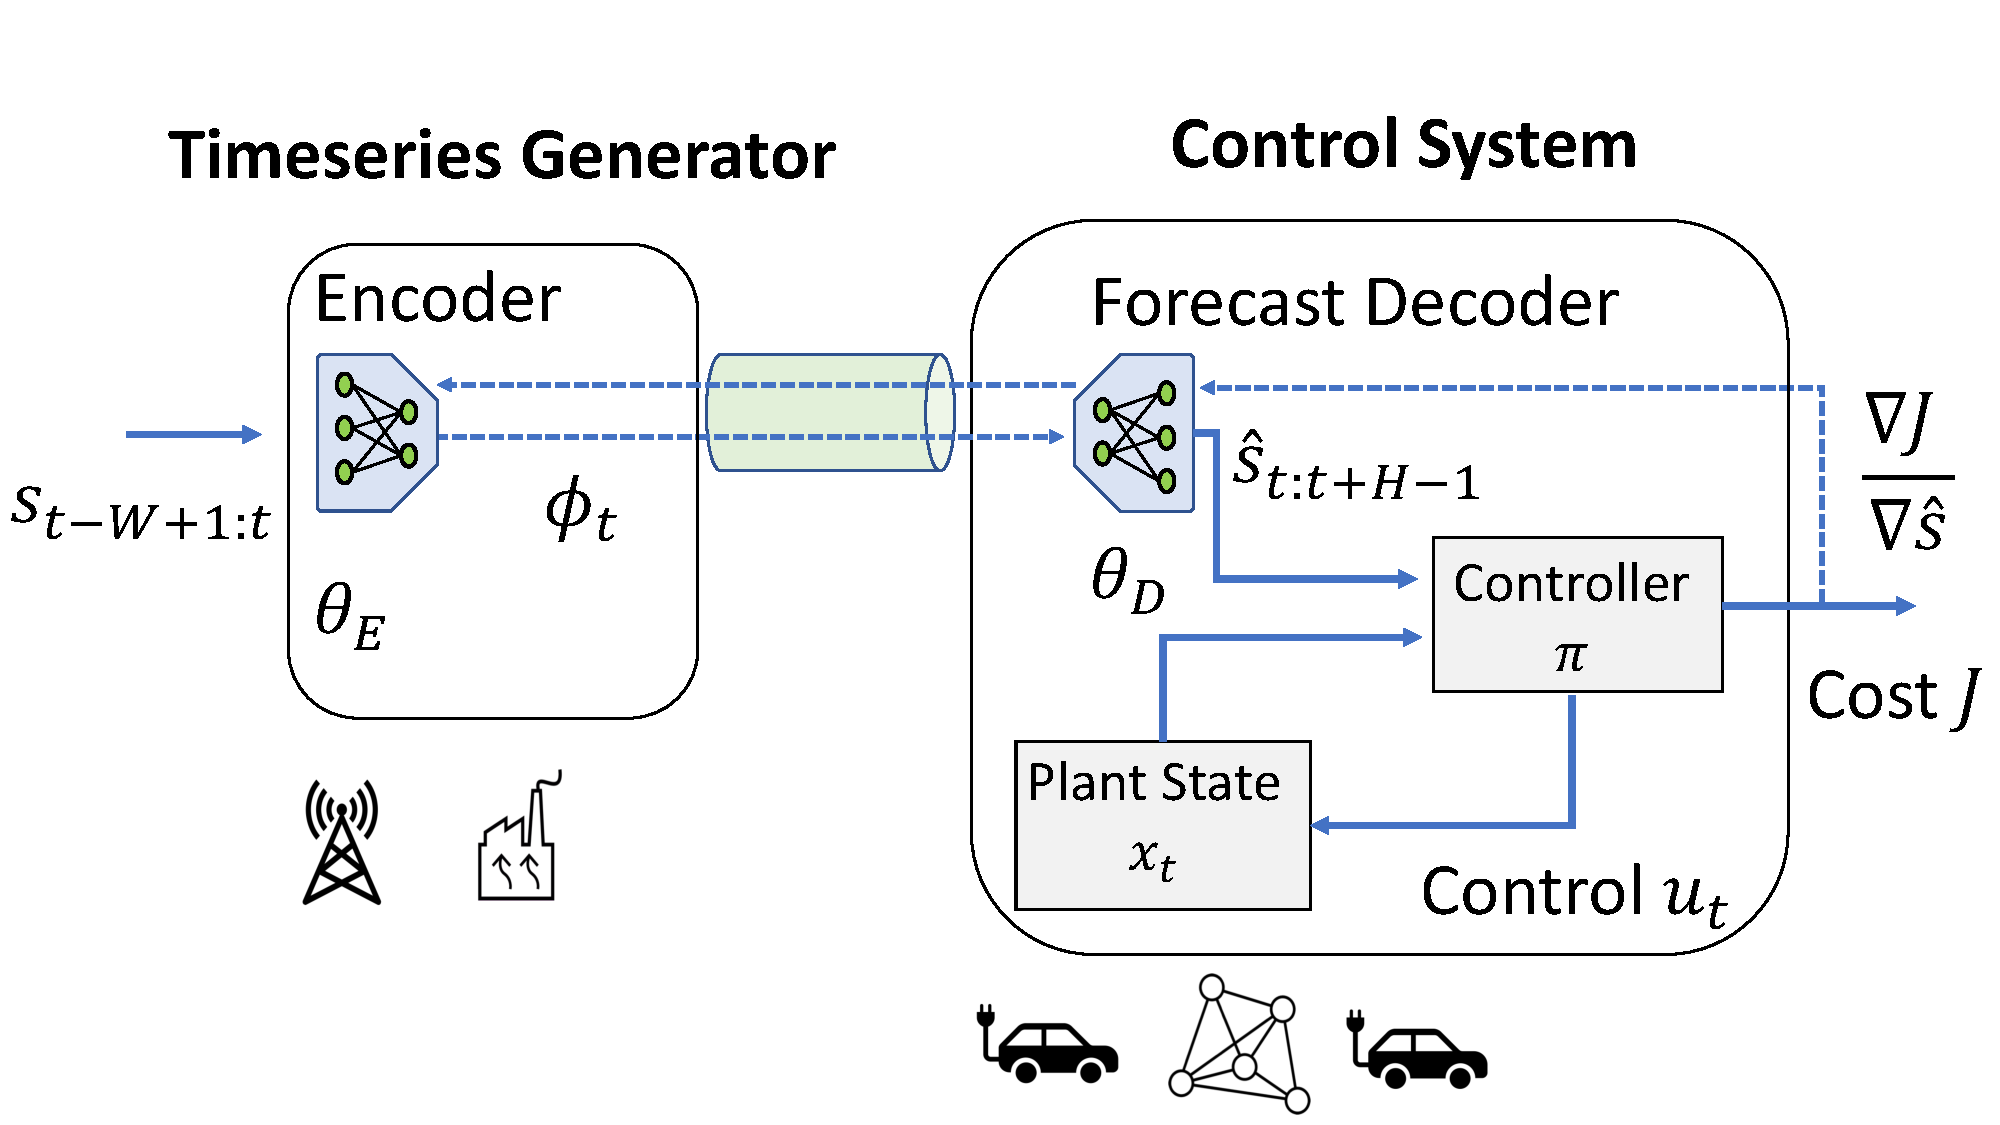
\includegraphics[width=0.99\columnwidth]{pics/final_model_nabla_2.pdf}
\caption{\textbf{Data sharing for cooperative control:} An owner of timeseries data $s_t$, such as a mobile operator, needs to transmit a compressed representation $\phi_t$ to a downstream controller with internal state $x_t$. The \textit{learned} forecast emphasizes task-relevant temporal features to minimize end-to-end controller cost $J$. \newline
    \SC{\textbf{Figure explanation: } This figure describes information flow and a similar figure should be referenced to introduce key notation in your problem formulation (at least for networking or control papers). Use white color and thick black lines as much as possible. Use color with a purpose. For example, all blue modules are learnable in the above figure, while grey modules are model-based. Describe key uses of color in the text or succinctly in the caption.}}
\label{fig_problem}
% \vskip -0.5em
\end{figure}


\subsection{Guidelines}

\subsubsection{Variables and Equations}

The following guidelines govern notation.

\begin{enumerate}
    \item \textbf{Time: } Use a subscript for \textit{discrete} time, such as $x_t$. A timeseries of variable $x$ from time $t_0$ to $t_f$ should be given by $x_{t_0:t_f}$.
    \item \textbf{Use Standard Notation: } In control, the state is generally given by $x_t$, control by $u_t$, policy by $\pi$, and cost function by $J$. Strictly follow the same notation as prior papers by Sandeep or key influential textbooks.
    \item \textbf{Intuitive Variable Choices: } Your reader has a limited attention span, and will forget random notation like $\psi, \Gamma$ unless it is necessary. Suppose we have $K$ epochs to run an algorithm. Instead of $K$, write $N_{\mathrm{epoch}}$, which is obvious in case I forget what $K$ is.
    \item \textbf{Deep Learning Notation: } Parameters of a model are given by $\theta$. If you have different models, call them $\theta_{\mathrm{enc.}}$, $\theta_{\mathrm{ctrl}}$ for an encoder and controller (for example), rather than use a slew of unintuitive varibles like $\alpha, \psi$ etc. Loss functions should be given by $\mathcal{L}$, datasets by $\mathcal{D}$, etc.
    \item Use $\textsc{mathrm}$ in LaTeX for English words in a LaTeX equation.
\end{enumerate}



